\documentclass[a4paper, 12pt, fleqn]{article}
\usepackage{libertine}
% \usepackage{setspace}%\setstretch{1.24} %Zeilenabstand �ndern
\usepackage[utf8]{inputenc} %Umlaute&Sonderzeichen einlesbar
\usepackage[normalem]{ulem}
\usepackage{amsmath,amssymb,amsthm}
\theoremstyle{definition}
\newtheorem{hyp}{H} 
\usepackage{natbib}
\setcitestyle{notesep={; }}

\usepackage[pdfborder={0 0 0}, breaklinks=true, hyperfootnotes=false, hypertexnames=false]{hyperref}
\usepackage{microtype}
\usepackage{booktabs}
\usepackage{graphicx}
\usepackage{pdflscape}
\usepackage{float}
\usepackage{pdfpages}
\usepackage{floatflt}
\newcommand{\symbolfootnote}[1]{\begingroup%
\renewcommand{\thefootnote}{\fnsymbol{footnote}}\footnote{#1}\endgroup}
\usepackage{array}
\newcommand{\inew}[1]{{\color{blue} #1\color{black}}}
\usepackage{comment}
\specialcomment{icomm}{\color{red}\footnotesize [\textsc{iren}: }{] \normalsize\color{black}}
\newcommand{\iout}[1]{{\color{red}\sout{#1}}}
%}
\newcommand{\old}[1]{{\color{lightgray} #1\color{black}}}

\newcommand{\mytitle}{{\Large \textsc{When personalization deters delegation to algorithms: Evidence from a preregistered experiment}}}

%opening
\title{\mytitle}
%\author{Wania Lefuloff}
\date{}

%Fuer Zeilenabstand
\usepackage{setspace}
%\doublespacing

%Fuer 1.5 inch margins
%\usepackage[a4paper]{geometry}
%\geometry{top=1.5in, bottom=1.5in, left=1.2in, right=1.2in}

\begin{document}
 
%  \maketitle
\thispagestyle{empty}
\begin{center}
	\mytitle\symbolfootnote{We are grateful to all the many people who helped us write this paper, first and foremost Chris Starmer and Robin Cubitt, to whom we owe several aspects of the design, as well as the lively research group at the TWI and participants of numerous workshops and conferences.}
  \vspace{.55cm}\\
 Lara Suraci \qquad\qquad\qquad Irenaeus Wolff\symbolfootnote{Corresponding author. Thurgau Institute of Economics, Hafenstrasse 6, 8280 Kreuzlingen, Switzerland, \textit{wolff@twi-kreuzlingen.ch}.}
\\\vspace{.25cm}
 \begin{small}
  \phantom{mortext}\textit{DG Cities \qquad\qquad Thurgau Institute of Economics \\ \phantom{moretext}\phantom{University} \qquad\qquad (TWI) / University of Konstanz} %University of Konstanz\\ Hafenstrasse 6, 8280 Kreuzlingen, Switzerland\\ wolff@twi-kreuzlingen.ch}
  \vspace{.03cm}\\
\vspace{.6cm}
 {This version: 27$^{\text{th}}$ April, 2026}
\vspace{.6cm}
\end{small}
\end{center}

\begin{abstract}
  Algorithmic decision aids increasingly act on users’ behalf, and in many instances users can either retain control or delegate decisions to an algorithm altogether. We test whether preference-based personalization increases or decreases willingness to delegate compared with an objective optimization criterion. In a preregistered between-subjects experiment (N = 233), participants repeatedly chose whether to decide themselves or to delegate to an algorithm. In one treatment, the delegation option is an optimization-based algorithm selecting the option with the highest expected value. In the other treatment, it is a preference-based (personalized) algorithm selecting according to participants’ previously elicited preferences. We find no evidence that preference-based personalization increases delegation relative to expected-value optimization throughout the task. Instead, personalization deters delegation in two ways. First, at first contact participants are significantly less likely to delegate to the preference-based algorithm than to the optimization-based algorithm; %this difference is confined to the very first decision and disappears immediately thereafter, with 
  in subsequent decisions, delegation rates are statistically indistinguishable across algorithm types. Second, categorical non-delegation (never delegating) is substantially more prevalent under preference-based personalization (15.7\%) than under objective optimization (3.4\%). 
  All in all, our results are consistent with the idea that preference-matching can raise initial hesitation and heighten concerns about personal autonomy and decision control for a subset of users, functioning as an acceptance barrier even when personalization is normatively appealing.
  
     \vspace{.25cm}
  \textit{Keywords:} {AI delegation, human-AI delegation, personalization, algorithm appreciation, algorithm aversion, trust in AI, financial decision-making, preregistered experiment.}\vspace{.15cm}
%  \\\textit{JEL:} {D81, C91, D83}
\end{abstract}
\vspace{-.5cm}

\section{Introduction}\label{sec:intro}
Algorithmic systems increasingly make and implement decisions on users’ behalf in both everyday and high-stakes contexts, from automated driving %and financial robo-advising 
to autonomous trading and smart-home control. Public perceptions of algorithmic decision-making vary substantially across domains and are shaped by perceived fairness, accountability, privacy, trust, and usefulness \citep{Aysolmaz2023}. In many such settings, users face a concrete choice: they can retain control and decide themselves, or delegate the decision to an algorithm. Delegation can reduce cognitive effort and simplify complex choice tasks, but it can also reshape perceived agency and responsibility for outcomes. Recent literature shows that people do delegate consequential choices to AI systems, and that this delegation depends on the decision context \citep{Candrian2022}. Note that throughout the paper, we refer to these systems interchangeably as algorithms, algorithmic advice, and algorithmic decision aids. This reflects the practical reality that, from a user's perspective, the boundary between AI and algorithmic decision rules is often opaque.

A common assumption is that \emph{personalization} should increase acceptance. If individuals differ in preferences, then a decision aid that incorporates those preferences should, in principle, deliver higher subjective utility than a one-size-fits-all rule. In financial decision support, for example, systems often elicit risk preferences and translate them into portfolio recommendations. The key empirical question, however, is not whether personalization sounds attractive in principle, but whether it actually increases willingness to delegate.

Existing evidence leaves that question open. In robo-advisor research, much of the evidence focuses on what predicts whether people adopt robo-advisors and how they use them \citep[for example,][]{Mahmud2025}, rather than on direct contrasts between preference-based personalization and objective delegation rules. Adjacent work has shown that giving users even slight control over an algorithm's output can increase adoption \citep{Dietvorst2018}, and that conversational onboarding and autonomy-preserving designs shape trust and uptake \citep{Hildebrand2021,Fink2024}. However, these studies vary the interface, degree of user control, or communication format---not the nature of the underlying decision rule itself. To our knowledge, no study has experimentally tested whether making an algorithm's decision rule preference-based, rather than objectively optimizing, changes actual delegation behavior. More generally, behavioral evidence shows that delegation to algorithms is shaped by more than expected performance: people sometimes avoid algorithms and sometimes prefer them based on the context \citep{Dietvorst2018,Logg2019}; they need to understand how recommendations are generated before accepting them \citep{Yeomans2019}; and acceptance depends on moderators such as perceived control and task features \citep{Mahmud2022,Chugunova2022}.

Preference-based personalization can therefore be double-edged. While it may increase perceived fit, it may also encroach on users' sense of choice authority: a system that claims to decide \emph{as you would} substitutes for personal judgment more directly than an impersonal optimization rule, making delegation feel like ceding active control rather than outsourcing a computation. Our own post-task evidence is consistent with this interpretation: many categorical non-delegators explicitly report wanting to \emph{keep} responsibility for the choice (but not the outcome), suggesting that the barrier is not fear of being held responsible but rather a positive valuation of exercising choice authority. This reading aligns with evidence that perceived control over one's choices---not just expected benefits---is a key driver of algorithm acceptance \citep{Schaap2024}. It also connects to findings that algorithmic transparency can paradoxically heighten resistance: disclosing how a system decides can trigger negative social interpretations \citep{Chen2024} and induce pushback in algorithmic management contexts \citep{Hu2024}, suggesting that transparency about a system's decision basis may itself contribute to a heightened sense of reduced agency.

These issues are especially salient at first contact, when users have no experiential basis for evaluating an algorithm and must judge based on abstract cues about its decision logic. Stable preferences for decision autonomy can constrain delegation even when delegation is instrumentally attractive \citep{Ivanova-Stenzel2025}, making the perceived loss of choice authority especially salient at the moment of delegation. Task characteristics matter too: trust and reliance depend on perceived objectivity and time pressure \citep{Yang2025}. Additionally, negative reactions to algorithmic errors are robust across different contexts and severity levels \citep{Renier2021}. Together, these factors suggest substantial initial skepticism about delegating to algorithms.

To understand what shapes these first-contact decisions, we must study observable behavior rather than attitudes alone. Behavioral reliance and self-reported trust need not coincide; evidence from AI-advisor interactions shows that determinants of behavioral trust can diverge from self-reported trust \citep{Schreibelmayr2025}. Moreover, even in repeated interaction settings, the mere framing of advice as AI-generated can produce systematic overreliance \citep{Klingbeil2024}, underscoring that label-driven cues persist beyond first contact. This motivates our focus on observable delegation behavior, treating first contact as a critical moment when abstract cues about an algorithm's decision logic are especially influential in shaping whether users delegate.

In this study, we contrast two decision rules that are both plausible in financial choice settings but may elicit different reactions. One algorithm follows an \emph{objective optimization rule} and selects the option with the highest expected value (EV), which may appear impersonal and easier to justify as a rule-based benchmark. The other is \emph{preference-based personalization} in a narrow sense: it predicts a participant's preferred choice from their previously elicited preferences rather than maximizing EV. In implementation terms, the personalized algorithm maps each participant's earlier choices in a simpler elicitation environment to corresponding choices in a more complex environment later in the experiment; it does not involve adaptive updating or learning during the delegation task.

To test this contrast, we run a preregistered between-subjects experiment with repeated delegation decisions. Participants first complete 12 binary lottery choices (Part 1), which provide the preference-elicitation input for the personalized algorithm. They then enter Part 2, where in each round they choose either to decide themselves among eight lottery options or to delegate that choice to the assigned algorithm (EV or preference-based, depending on the treatment). 

This design allows us to isolate a preregistered first-contact test, before any outcome feedback is observed, and to distinguish it from behavior after feedback has accumulated. 
The comparison between our algorithms connects to evidence that responsibility-sharing considerations can shape advisor choice in human-versus-algorithm settings \citep{Gazit2023} and to recent studies of financial delegation and outcome evaluation \citep{Ismagilova2025}. Related findings in financial delegation are also suggestive of responsibility-sharing considerations \citep{Werner2026}, even though evidence on perceived responsibility differences between human and machine partners is mixed \citep{Kirchkamp2019}.

\subsection*{Preregistered hypothesis and analysis plan}
Consistent with our preregistration ({\scriptsize\url{https://aspredicted.org/7un5qf.pdf}}), the main hypothesis is: 
\begin{hyp}
	People are more likely to delegate financial decisions to an EV-maximizing algorithm than to a personalized algorithm that incorporates their (revealed) preferences.
\end{hyp}

Our preregistered primary analyses test this hypothesis in two complementary ways. First, we test the treatment difference in delegation in the first decision (round 1) using a one-sided Boschloo exact test. This isolates first contact, when participants have no outcome feedback and must decide whether to delegate based on their interpretation of the algorithm. Second, we test whether EV maximization leads to higher delegation overall by comparing participants' average delegation frequencies across rounds using a one-sided Wilcoxon--Mann--Whitney test.

To account for the repeated-decision structure and additional determinants of delegation, our preregistration also specifies a multivariate regression analysis. We estimate a model with treatment indicators interacted with the decision period, decision-ID fixed effects, and participant-clustered standard errors. We further include the feedback history in the form of including the share of zero outcomes among prior delegated choices, to control for how experienced payoffs may influence subsequent delegation decisions. This preregistered specification tests whether any treatment difference varies systematically over decisions while controlling for option-set heterogeneity and participants' feedback histories.

\subsection*{Study overview and supplementary analyses}
We implement our design in a between-subjects experiment in which participants repeatedly choose whether to decide themselves or delegate to the assigned algorithm. The repeated-decision setting provides a direct behavioral measure of delegation and allows us to distinguish first-contact delegation from later decisions.

In addition to the preregistered tests, we report a small set of analyses to characterize heterogeneity in delegation propensity. In particular, we examine categorical non-delegation (never delegating across rounds). This outcome captures a distinct form of resistance to algorithmic control transfer and is relevant for understanding which users may opt out of decision aids altogether.

In sum, this paper provides a preregistered test of a simple but consequential claim: even in a setting where preference-based personalization may appear normatively attractive, people may nonetheless be more willing to delegate to a `more objective' algorithm. The contribution is threefold: we provide a preregistered behavioral comparison of objective versus personalized decision rules, we identify where the treatment effect is concentrated (first contact), and we document categorical non-delegation as a distinct uptake barrier under personalization. Together, these findings sharpen the design implication that uptake depends on perceived rule characteristics, not only on expected performance.




A common assumption is that personalization should increase acceptance \citep{DeanMorgenstern2022}. If individuals differ in preferences, then a decision aid that incorporates those preferences should, in principle, deliver higher subjective utility than a one-size-fits-all rule. In financial decision support, for example, systems often elicit risk preferences and map them to recommended portfolios. However, behavioral evidence suggests that willingness to use algorithmic advice is not determined by instrumental considerations alone. People sometimes avoid algorithms, sometimes prefer them, and often react to how they interpret a system’s role and legitimacy (e.g., Dietvorst et al., 2015; Logg et al., 2019; Castelo et al., 2019). Preference-based personalization can therefore be double-edged: while it promises better fit, it can also make the system’s decisions traceable to a user profile, potentially heightening discomfort with being categorized or increasing perceived responsibility for outcomes (“it chose based on me”).
%
%These issues are especially salient at first contact, when users have no experiential basis for evaluating an algorithm. At first contact, delegation is likely to depend on abstract cues about what an algorithm optimizes and what that implies about the user, rather than on experienced accuracy. Therefore, early impressions and system descriptions can shape adoption and reliance even when objective performance is held constant (e.g., Kosch et al., 2022). Moreover, self-reported trust and behavioral reliance often diverge (Papenmeier et al., 2022), which motivates studying delegation as an observable behavior rather than equating it with stable trust. 
%
%In this study, we contrast two decision rules that are both plausible in financial choice settings but may elicit different reactions. One algorithm selects the option with the highest expected value (EV), a rule that may appear impersonal and objectively justified. The other is preference-based (“personalized”) in a narrow sense: it selects options according to participants’ previously elicited (revealed) preferences rather than by optimizing EV. Here, “personalized” refers to profile-based selection from elicited preferences, not to online learning or continuous adaptation. The central question is whether people are more willing to delegate to EV maximization than to preference-based personalization.
%
%Preregistered hypothesis and analysis plan
%
%Consistent with our preregistration, the main hypothesis is:
%
%H1 (Preregistered). People are more likely to delegate financial decisions to an EV-maximizing algorithm than to a personalized algorithm that incorporates their (revealed) preferences.
%
%Our preregistered primary analyses test this hypothesis in two complementary ways. First, we test the treatment difference in delegation in the first decision (round 1) using a one-sided Boschloo exact test. This isolates first contact, when participants have no outcome feedback and must decide whether to delegate based on their interpretation of the algorithm. Second, we test whether EV maximization leads to higher delegation overall by comparing participants’ average delegation frequencies across rounds using a one-sided Wilcoxon–Mann–Whitney test.
%
%To account for the repeated-decision structure and additional determinants of delegation, our preregistration also specifies multivariate regression analyses. We estimate models with treatment indicators interacted with the decision period, decision-ID fixed effects, and participant-clustered standard errors. We further include measures capturing feedback history, including the share of zero outcomes among prior delegated choices, to control for how experienced payoffs may influence subsequent delegation decisions. This preregistered specification tests whether any treatment difference varies systematically over decisions while controlling for option-set heterogeneity and participants’ feedback histories.
%
%Study overview and supplementary analyses
%
%We implement this design in a preregistered between-subjects experiment in which participants repeatedly choose whether to decide themselves or delegate to the assigned algorithm. The repeated-decision setting provides a direct behavioral measure of delegation and allows us to distinguish first-contact delegation from later decisions made after minimal experience.
%
%In addition to the preregistered tests, we report a small set of analyses to characterize heterogeneity in delegation propensity. In particular, we examine categorical non-delegation (never delegating across rounds). This outcome captures a distinct form of resistance to algorithmic control transfer and is relevant for understanding which users may opt out of decision aids altogether. 
%
%In sum, this paper provides a preregistered test of a simple but consequential claim: even in a setting where preference-based personalization may appear normatively attractive, people may nonetheless be more willing to delegate to an EV-maximizing algorithm. Our design and preregistered analyses allow us to assess this claim both at first contact and on average across repeated decisions, and show that resistance to personalization can take the form of both first-contact hesitation and categorical non-delegation.


\section{Related Work}
\label{sec:related}

Our work sits at the intersection of literatures on (i) the behavioral uptake of algorithmic decision aids, (ii) delegation, agency, and responsibility in human--algorithm interaction, (iii) transparency as an interpretive cue for acceptance, (iv) personalization as a design feature of algorithmic decision rules, and (v) heterogeneity in trust and delegation. Below, we situate our study within these streams, identify the specific gap our experiment addresses---the lack of a direct behavioral comparison between personalized and objective decision rules---and connect them to the robo-advisor application domain.

\subsection{Algorithm aversion, appreciation, and conditions for uptake}
Behavioral uptake of algorithmic advice is not one-directional: studies document both \emph{algorithm aversion} and \emph{algorithm appreciation}, depending on context, feedback, and comparison benchmark \citep{Dietvorst2018,Logg2019}. A core implication is that reliance cannot be predicted based on objective performance alone. Users need to make sense of how recommendations are generated before accepting them, and understandability can gate uptake independently of accuracy \citep{Yeomans2019}. Systematic evidence further shows that uptake is moderated by factors at multiple levels (algorithm, individual, and task), including perceived control and decision context \citep{Mahmud2022,Chugunova2022}.

This mixed-evidence baseline motivates our design choice to study delegation as an observed behavioral outcome and to isolate one concrete determinant of uptake: the algorithmic \emph{decision rule} (objective EV maximization versus preference-based personalization).

\subsection{Delegation, agency, and responsibility sharing}
Delegation goes beyond advice-taking: it is a transfer-of-control decision that entails ceding choice authority to the algorithm \citep{Candrian2022}. For that reason, agency and responsibility become central concerns. In advisor-choice settings, people evaluate more than expected payoff, including whether responsibility for consequences can be shared with or offloaded onto the advisor \citep{Gazit2023}. Related evidence from financial delegation suggests that delegation patterns are consistent with responsibility-sharing motivations, particularly in loss contexts \citep{Werner2026}. Yet, evidence on whether perceived responsibility differs between human and machine partners is mixed, with \citet{Kirchkamp2019} finding little difference in perceived responsibility or guilt.

This control-and-responsibility perspective is consistent with adjacent evidence: perceived trustworthiness dimensions shape acceptance of algorithmic decision-makers \citep{Hoeddinghaus2021}; preserving human involvement can increase uptake but may lower accuracy \citep{Sele2024}; and stable preferences for decision autonomy can constrain delegation even when delegation is instrumentally attractive \citep{Ivanova-Stenzel2025}. Taken together, this evidence implies that delegation is shaped by perceived control and responsibility allocation, not only expected returns. This motivates our focus on observed delegation behavior and makes the EV-versus-personalized comparison directly informative, because the two rules differ in how strongly they cue impersonal objectivity versus personal ownership of outcomes.

\subsection{Transparency, and interpretive cues for acceptance}
Personalization and transparency are often presented as acceptance-enhancing design features, but recent evidence suggests they can also trigger resistance. In recommendation contexts, greater transparency can backfire when users infer socially negative meanings (for example, feeling judged or dehumanized), reducing acceptance \citep{Chen2024}. In algorithmic management, transparency can likewise show a non-monotonic effect, where additional transparency eventually increases resistance rather than compliance \citep{Hu2024}. Related evidence further indicates that acceptance is driven less by whether the decision-maker is labeled algorithmic or human, and more by expected benefits and perceived control \citep{Schaap2024}.

The broader explainability literature is consistent with this interpretation: transparency and explanations matter, but their effects depend on what they change psychologically. Fairness/accountability/transparency perceptions shape trust and adoption \citep{Shin2019}; explanations can improve trust calibration and behavior in some settings \citep{Leichtmann2023}; and combining explanation with decision control can improve compliance, though design complexity can also offset those gains \citep{Westphal2023}. In applied decision-support experiments, transparency influences advice use via trusting beliefs and perceived understanding, with effects that depend on the information environment and experienced system performance \citep{Ning2024,Sun2026}. For our setting, this implies that users' interpretation of decision logic can shape delegation independently of objective expected returns.

\subsection{Decision-rule comparison gap: personalized versus objective rules}
Despite the breadth of the literatures reviewed above, a striking gap remains: to our knowledge, no study has experimentally tested whether making an algorithm's decision rule \emph{preference-based} (as opposed to following an impersonal, objective criterion) changes actual delegation behavior. Several lines of work come close but address different questions.

First, the ``algorithm modification'' paradigm pioneered by \citet{Dietvorst2018} shows that giving users even slight control over an algorithm's output increases adoption. This demonstrates that \emph{user input} matters, but the manipulation concerns users' ability to adjust the output, not whether the underlying decision rule incorporates their preferences or maximizes an objective criterion.

Second, the robo-advisor design literature examines how features such as conversational onboarding \citep{Hildebrand2021}, user controllability over rebalancing \citep{Kim2025ICIS}, and the performance--control trade-off in configuration choices \citep{Ruehr2020} shape adoption and trust. These studies vary the \emph{interface} and the \emph{degree of control}, but hold the nature of the decision rule itself constant or leave it as an implicit design feature.

Third, theoretical and empirical work on robo-advisor personalization has focused on optimizing portfolio allocation through more granular client interaction \citep{Capponi2022} or on comparing algorithm-selected portfolios with self-directed choices \citep{BouluReshef2026}. These contributions are informative about \emph{performance} implications of personalization, but do not ask whether users are more or less willing to delegate when the algorithm's rule is personalized.

This gap is consequential beyond academic interest. In practice, financial robo-advisors, healthcare decision aids, and algorithmic recommender systems routinely face the design choice between objective optimization criteria (such as expected-value or evidence-based guidelines) and preference-based rules that incorporate individual user profiles. If personalization reduces rather than increases the willingness to delegate---as our evidence suggests---then system designers may inadvertently raise adoption barriers by prioritizing preference-matching. Understanding this trade-off is directly relevant for any domain where algorithmic decision aids must be voluntarily adopted to be effective.

\subsection{Heterogeneity and contextual moderators of trust and delegation}
Recent evidence shows that algorithm uptake is heterogeneous across people, tasks, and decision environments \citep{Ferraz2025,Yang2025}. At the individual level, delegation varies with psychological readiness and other personal traits linked to delegation behavior \citep{Kim2026,Ferraz2025}. Beyond stable traits, uptake also depends on decision architecture: autonomy-preserving choice designs can increase recommendation acceptance \citep{Fink2024}. At the task level, uptake depends on objectivity and time pressure \citep{Yang2025}, while overreliance risks remain salient when users follow advice against their own information \citep{Klingbeil2024}. Taken together, these cross-level moderators imply that average delegation rates can mask meaningful subgroup patterns. For our study, this motivates looking beyond means and explicitly reporting categorical non-delegation as a distinct acceptance pattern.

\subsection{Financial advice and robo-advisors as an application domain}
Although our task is experimentally stylized, it maps naturally to financial delegation settings where users decide whether to retain control or hand choice authority to an algorithmic decision aid. This is exactly the context in which objective optimization and preference-based personalization often coexist in practice. Existing robo-advisor evidence is informative but fragmented: studies document adoption patterns and how users combine advisor recommendations with their own judgment \citep{Figa-Talamanca2022,Mahmud2025}, outcome bias in the evaluation of delegated financial decisions, whether made by a human or an algorithm \citep{Ismagilova2025}, and potential performance gains from robo-advice relative to self-directed choices \citep{Lambrecht2023}. 

This makes financial decision-making a strong test bed for our question: whether changing the algorithmic decision rule changes willingness to delegate, even when both rules are plausible.

\subsection{Synthesis and contribution}
Across these literatures, the common message is that delegation to algorithms is jointly shaped by decision-rule design, perceived control and responsibility, trust calibration, and context-dependent interpretation of transparency and autonomy-related design cues \citep{Dietvorst2018,Chugunova2022,Schaap2024,Fink2024,Hu2024}. Yet as we have documented above, the existing evidence base contains a notable gap: while adjacent work has studied algorithm modification, controllability, conversational design, and performance implications of personalized portfolios, no study has experimentally isolated the effect of the decision rule itself---specifically, whether making the rule preference-based rather than objectively optimizing changes users' willingness to delegate. This gap matters practically because robo-advisors, healthcare decision aids, and algorithmic recommender systems routinely face exactly this design choice, and a wrong assumption about the direction of the effect could raise rather than lower adoption barriers.

Our study addresses this gap with a preregistered behavioral test in a repeated-decision delegation paradigm, contrasting an EV-maximizing rule with a preference-based rule. By jointly examining first-contact delegation, average delegation across rounds, and categorical non-delegation, we connect classic aversion/ appreciation evidence with newer findings on autonomy, transparency backfire, and responsibility attribution \citep{Logg2019,Fink2024,Hu2024,Gazit2023}.

\section{Method}
\label{sec:method}

\subsection{Participants and preregistered exclusions}
Participants were recruited via Prolific from a UK-based participant pool and completed the study online. The preregistered target was 120 participants per treatment condition before exclusions. We recruited N = 240 participants and then applied preregistered exclusion rules for data quality and protocol compliance. Exclusions covered failed bot/slider checks at first attempt, failed comprehension checks after the second attempt, failure to confirm careful participation, disclosed AI usage during the study, implausibly short completion times under the preregistered log-time rule, and incomplete data. The final analysis sample is N = 233 (EV condition: n = 118; preference-based condition: n = 115).

\subsection{Design and task}
The study used a between-subjects design with two algorithm conditions. In both conditions, participants completed a two-part experiment programmed in the online-ready version of z-Tree \citep{Fischbacher07}.

Part 1 consisted of 12 binary lottery choices used to elicit revealed risk preferences. Eight of these tasks were directly linked to Part 2 (see below); the remaining four served as filler tasks as one of several measures to prevent participants from anticipating the structural correspondence between Part 1 and Part 2. Participants were truthfully told that ``[t]he questions in this part are \textbf{hypothetical}, but the choices \textbf{may be meaningful for Part 2} (recall that your bonus payment from the experiment depends on what happens in Part 2).'' The highlighted words were boldfaced in the original instructions. In Part 1, payoffs were matched to states so that they would appear in decreasing order to ease comparison, as can be seen in the upper panel of Figure \ref{fig:example_screens}. In addition, we asked participants after each task in Part 1 how confident they were in their choice.

In Part 2, participants completed eight incentivized decisions between eight lottery options each. These eight Part-2 tasks were derived from eight mapped Part-1 binary tasks (all but the four filler tasks). Specifically, each mapped Part-1 task provided two ``anchor'' options; for Part 2, we first transformed each anchor option by permuting payoffs across states (Option 6 and Option 3 in the lower panel of Figure \ref{fig:example_screens}), and then added three decoy options for each anchor option---options that were dominated by one of the anchor options (i.e., worse in at least one outcome and no better in any other), without making the dominance relationship immediately obvious from the displayed payoffs. This yields eight options per Part-2 task (two transformed anchors plus six decoy options). The within-task display order of the eight options was set using a fixed pre-specified rule rather than per-task randomization. We did this because unconstrained randomization would occasionally produce display orders where the three decoy options belonging to the same anchor would appear consecutively next to the anchor option itself---a clustering that could alert attentive participants to the underlying construction logic of Part-2 tasks. The fixed ordering rule was designed to interleave anchor-based groups so that no such visually suspicious pattern would arise and was different between option sets.

The order of the 12 Part-1 tasks was randomized with one pre-defined constraint: positions 11 and 12 were occupied by two (randomly selected) tasks from the four Part-1 filler tasks that had no mapped counterpart in Part 2. Consequently, all eight mapped Part-1 tasks appeared within the first ten Part-1 positions, while still preserving randomization of task order subject to this constraint.

\begin{figure}[htbp]
\centering
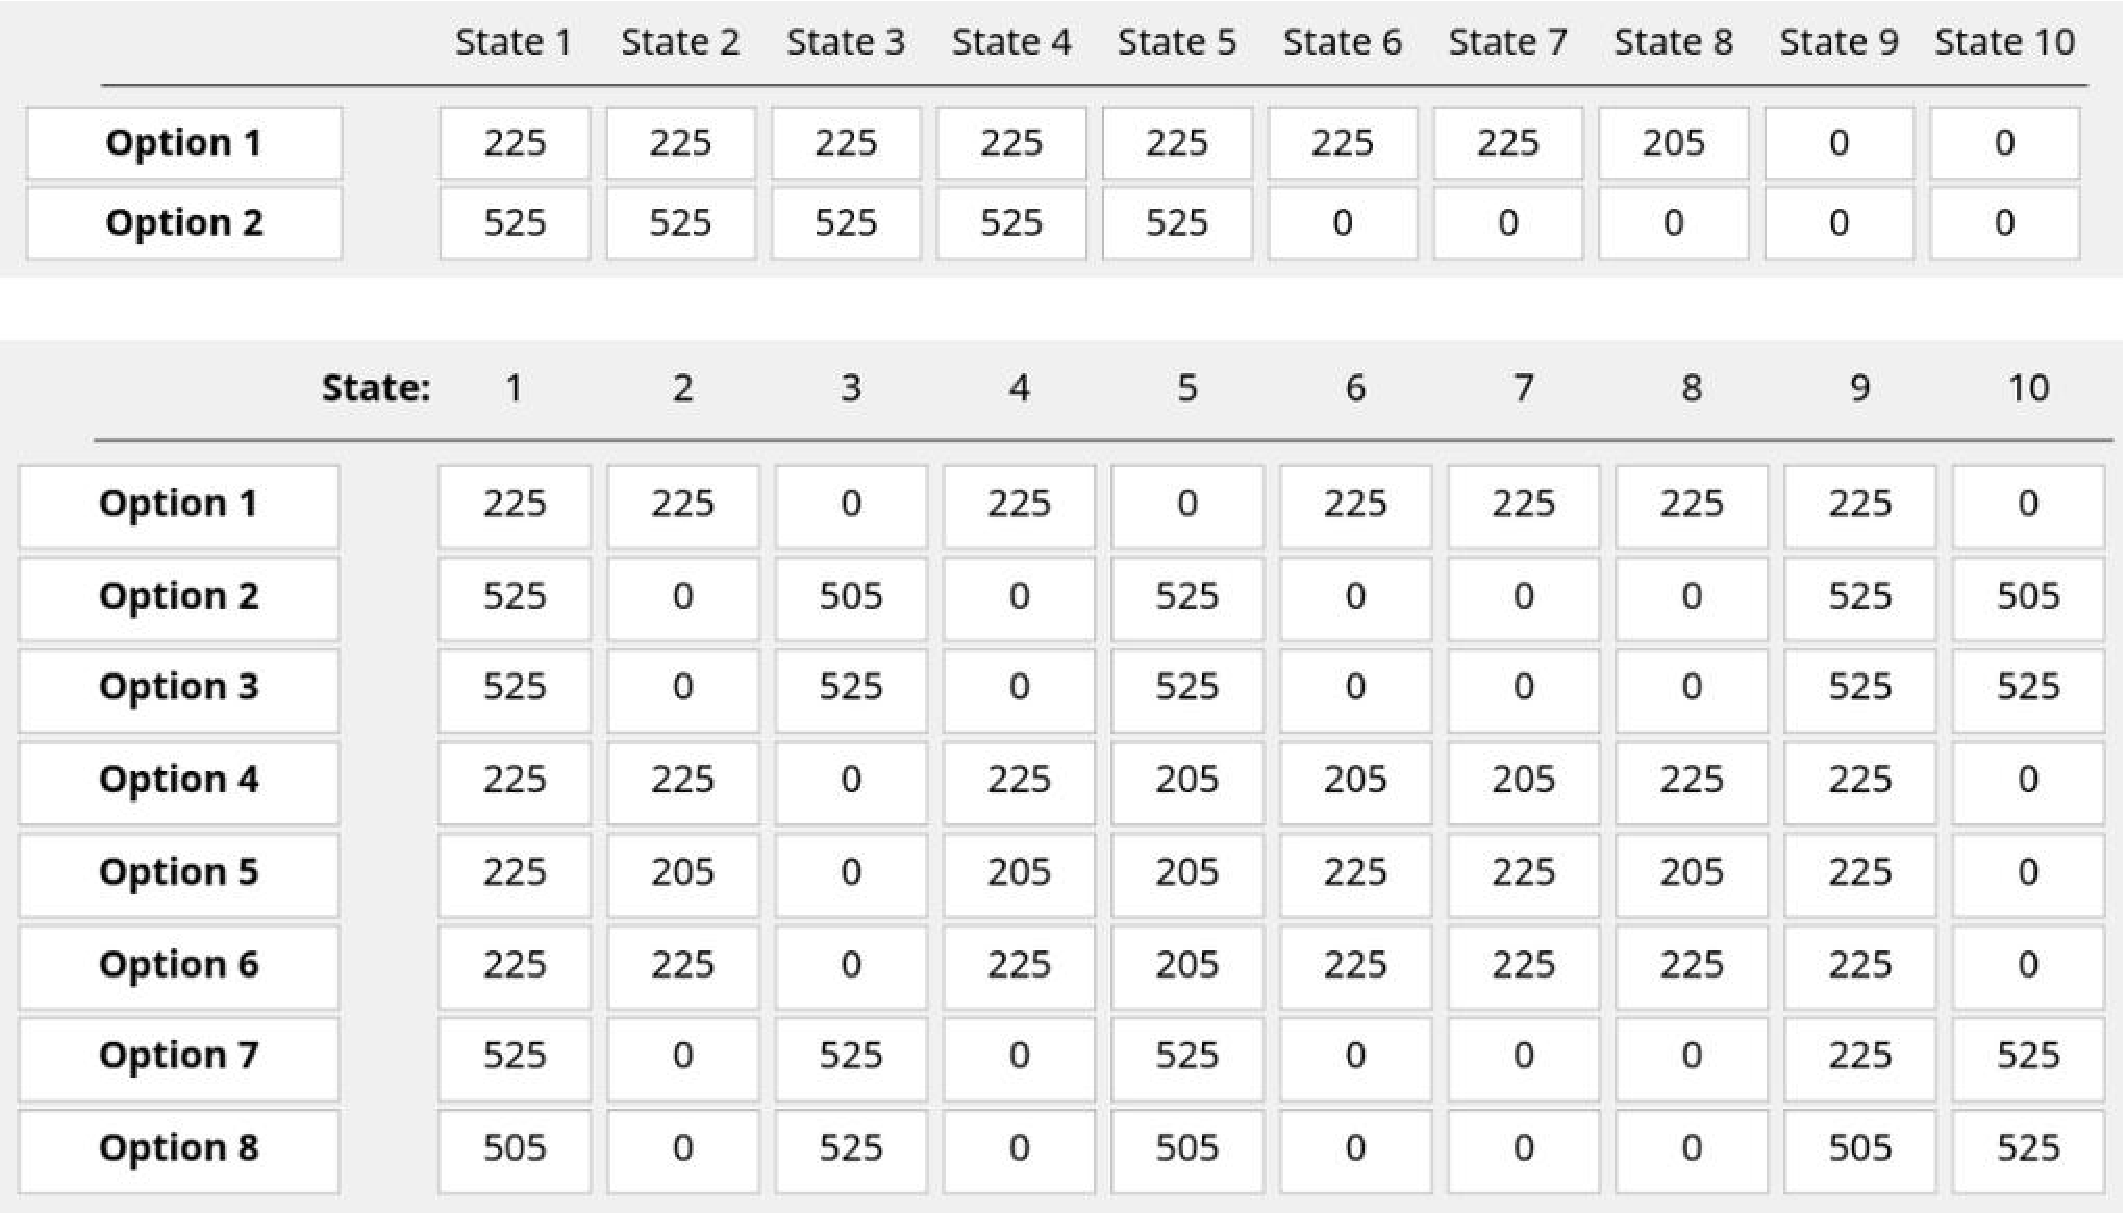
\includegraphics[width=0.85\textwidth]{Figure_ExampleScreens.pdf}
\caption{Example screens from Part 1 (preference elicitation, upper panel) and Part 2 (delegation decisions with lottery choices, lower panel).}
\label{fig:example_screens}
\end{figure}

The procedure for each round of Part 2 was as follows: Participants saw the full table for five seconds. Then, they saw a different screen on which they had five seconds to choose between delegating to the algorithm corresponding to their treatment condition and choosing an option themselves.
In the EV condition, delegation selected the lottery with the highest expected value. In the preference-based condition, delegation followed each participant's elicited preference profile from Part 1. Importantly, in both treatments the delegated option was always one of the two transformed anchor options and therefore never one of the six decoy options. Assignment to condition was randomized at the participant level. In the EV condition, participants were informed that ``[the] algorithm works out how much each option would yield on average, and selects the option for which this is highest.'' In the preference-based condition, they instead read that ``[the] algorithm analyses your choices from Part 1 and selects the best option for you in light of your Part-1 choices.''

If they did not delegate, they saw the table containing the eight options for up to eight more seconds, during which they had to choose one of the options. After each Part-2 decision, feedback provided full resolution of uncertainty: participants were shown the chosen option and the realized payoff from one randomly drawn state of the world for that round. If they did not make a choice in the payoff-relevant task, they did not earn a bonus payment from the experiment. The total payoff from the experiment was GBP 2.00 plus the points earned in one randomly selected round of Part 2, converted at a rate of 1 penny per point (participants could earn up to GBP 8.90 in addition to the base payoff). On average, participants earned GBP 4.14 including the base payoff for a median time of just under 16 minutes.

\subsection{Procedure}
After consent, participants completed attention and comprehension checks, then Part 1 (preference elicitation), followed by a question on how satisfied they were with their choices from Part 1 overall. Then, participants completed Part 2 (delegation decisions with round-by-round outcome feedback), followed by a question of whether they would delegate to the algorithm in case they had to choose to delegate or not for 10 (hypothetical) additional tasks. After indicating that choice, participants estimated (on a 0--10 integer scale) in how many of those 10 tasks the algorithm would choose a non-preferred option and in how many it would choose a ``completely weird'' option. Before the final post-task questionnaire containing demographics and attitudinal items, we asked them for self-reported reasons for their choice in the hypothetical choice at the end of Part 2. Because our theoretical focus is reliance behavior, primary outcomes are behavioral rather than attitudinal.

\subsection{Ethics approval}
The study received ethics approval from the Institutional Review Board of the Gesellschaft für experimentelle Wirtschaftsforschung e.V. (GfeW; German Association for Experimental Economic Research), certificate no. 19HBJNwQ (status: approved; expedited review; approval date: 11/13/2025; certificate validity through 11/13/2027; see {\footnotesize\url{https://gfew.de/ethik/19HBJNwQ}}). All participants provided informed consent before participation.

\subsection{Preregistered outcomes and analyses}
The preregistered hypothesis (H1) predicted higher delegation to the EV-maximizing algorithm than to the preference-based algorithm.
The preregistration document is available at {\footnotesize\url{https://aspredicted.org/7un5qf.pdf}}.

Primary preregistered analyses were:
\begin{enumerate}
  \item a one-sided Boschloo exact test for the treatment difference in delegation in round 1 (first contact), and
  \item a one-sided Wilcoxon--Mann--Whitney test comparing participant-level average delegation rates across Part 2.
\end{enumerate}

We additionally estimated a preregistered linear probability model with decision-set fixed effects and participant-clustered standard errors, including treatment-by-period interactions and the share of outcomes with a payoff of zero among prior delegated choices. We further estimated an exploratory specification excluding round 1 to separate first-contact effects from choices made after feedback experience.

\section{Results}
\label{sec:results}

\subsection{Overview}
Two empirical patterns organize the results. First, treatment differences are concentrated at first contact. Second, categorical non-delegation is substantially more common under preference-based personalization.

\subsection{Primary test: first-contact delegation}
As a benchmark for interpreting delegation behavior, choice quality among non-delegated decisions was low in both treatments. The share of non-dominated self-chosen options was 34.1\% in the EV condition and 35.1\% in the preference-based condition, implying that roughly two-thirds of self-made choices were dominated. Hence, participants had a clear instrumental reason to delegate. On average, delegated decisions yielded 243.49 points (GBP 2.43), compared to 195.18 points (GBP 1.95) for non-delegated decisions, a difference of approximately 25\%.

In round 1, delegation was higher in the EV condition than in the preference-based condition (66.9\% vs. 55.8\%). The preregistered one-sided Boschloo exact test yields p = 0.0413, supporting H1 for first-contact behavior.
Figure~\ref{fig:average_delegation_over_time} visualizes the round-level profile and shows that the treatment gap is concentrated in the first decision.

\begin{figure}[tb]
	\centering
	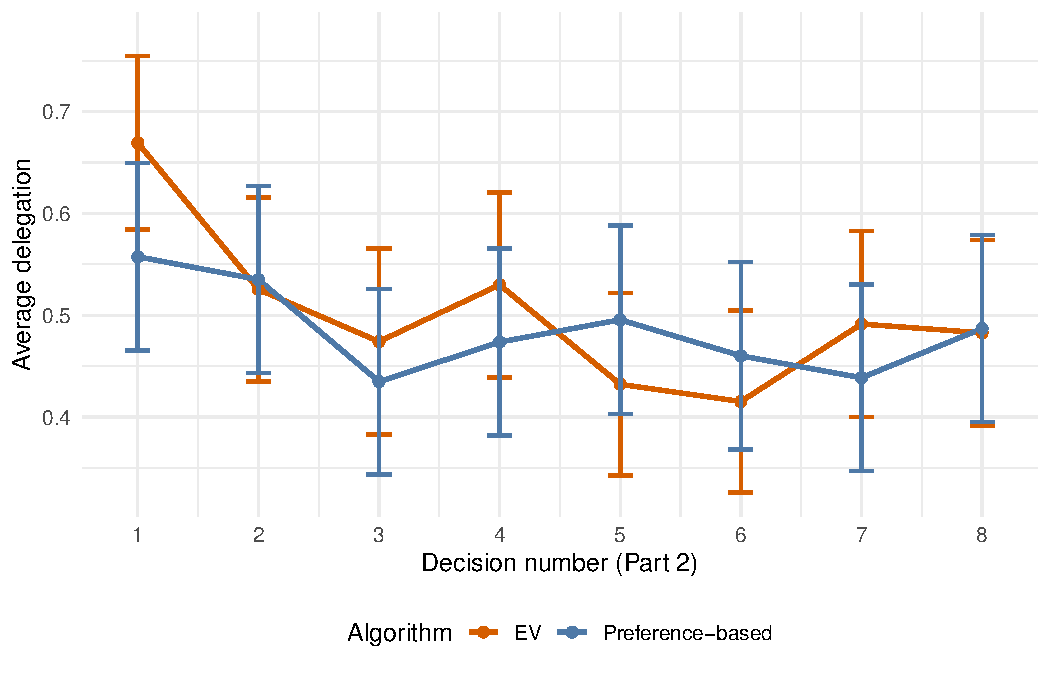
\includegraphics[width=0.8\textwidth]{Figure1_AverageDelegation.pdf}
	\caption{Average delegation over decisions in Part 2 by treatment condition.}
	\label{fig:average_delegation_over_time}
\end{figure}

\subsection{Primary test: delegation across repeated decisions}
At the participant level, the preregistered one-sided Wilcoxon--Mann--Whitney test on average delegation across Part 2 yields W = 6428 and p = 0.2425. We therefore do not find evidence of a treatment difference in average delegation across rounds.

Descriptively, this non-difference reflects post-first-contact convergence that is driven more by a stronger decline in delegation in the EV condition after round 1 than by additional declines in the preference-based condition (Figure~\ref{fig:average_delegation_over_time}). We treat this pattern as descriptive because our design was not optimized to identify why EV delegation appears more sensitive to early feedback after first contact.

The preregistered regression specification points in the same direction. The EVAlgorithm coefficient is small and statistically insignificant ($\beta = -0.0487$, SE = 0.0831, $p = 0.558$). Likewise, both interaction terms are imprecisely estimated (EVAlgorithm $\times$ WithinPartDecisionNumber: $\beta = 0.0019$, SE = 0.0115, $p = 0.871$; EVAlgorithm $\times$ share[Payoff $= 0$]: $\beta = -0.0497$, SE = 0.0977, $p = 0.612$), indicating no robust treatment difference over repeated decisions. By contrast, the share of prior delegated outcomes with a payoff of zero is strongly negatively associated with subsequent delegation ($\beta = -0.3854$, SE = 0.0781, $p < 0.001$).\footnote{Running an analogous regression with fixed effects for the task on round-1 data only yields the same result as the Boschloo test, with $\beta = 0.113$, SE = 0.065, and $p = 0.041$ (one-sided).}

Taken together, the preregistered tests indicate that the treatment effect is concentrated at first contact and does not persist over repeated decisions, while negative feedback (in particular prior zero-outcomes) is strongly associated with lower subsequent delegation. The convergence in delegation behavior over rounds is visible in Figure~\ref{fig:average_delegation_over_time}; the cross-participant distribution is shown in Figure~\ref{fig:delegation_ecdf}. This does not diminish the substantive relevance of first-contact effects: in many real settings, the initial adoption decision can determine whether users return to a system at all.

\begin{figure}[tb]
	\centering
	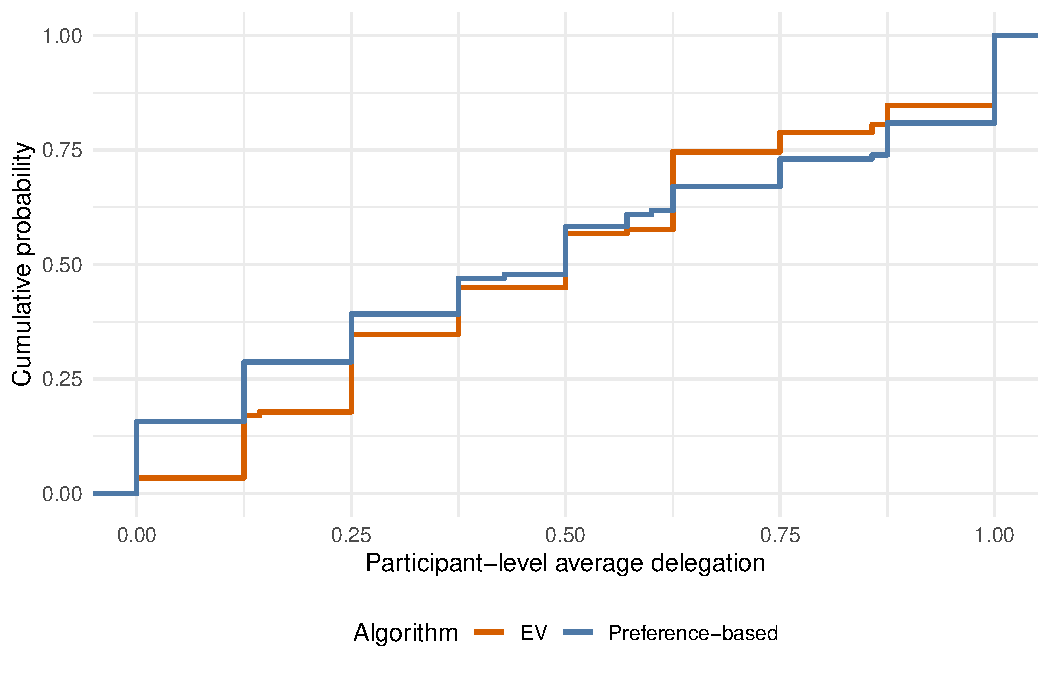
\includegraphics[width=0.78\textwidth]{Figure3_ECDF.pdf}
	\caption{ECDF of participant-level average delegation by treatment condition.}
	\label{fig:delegation_ecdf}
\end{figure}

\subsection{Categorical non-delegation}
This section reports an outcome that was not preregistered (categorical non-delegation) that is complementary to the preregistered primary tests.

The second clear pattern is categorical non-delegation, which can be seen from the left end of Figure~\ref{fig:delegation_ecdf}. In the preference-based condition, 18 of 115 participants never delegated (15.7\%); in the EV condition, this applies to only 4 of 118 participants (3.4\%). This gap points to a distinct acceptance barrier under personalization for a subset of users.\footnote{The same direction appears in an earlier study with a different design (reported in Suraci's PhD thesis): 32/189 never-delegators in preference-based treatments versus 17/187 in EV treatments (one-sided Boschloo exact test, $p = 0.0135$).} Note that although there also seems to be a treatment difference in always-delegators, this difference is far less pronounced (19.1\% vs. 13.6\%).

Never-delegators were not meaningfully different in age from participants who delegated at least once (mean age 41.8 vs. 42.9 years; $t = -0.329$, $p = 0.745$), and we likewise find no clear association with household income (categorical; \(\chi^2\) = 13.171, df = 11, p = 0.282) or education (categorical; \(\chi^2\) = 1.859, df = 5, $p = 0.868$), and both spent similar amounts of time in the experiment (mean number of seconds 1113 for delegators vs. 1237 for never-delegators, $t = -0.971$, $p = 0.341$). And while there is a tendency for male participants to be never-delegators more often than females (12.0\% vs. 6.3\%), the evidence is weak (Boschloo exact test, $p = 0.156$). We also do not find meaningful differences in self-reported willingness to take financial risks (4.53 vs. 4.68; $t = -0.224$, $p = 0.825$), self-reported response reliability/care (Reliable: 6.91 vs. 6.91; $t = -0.059$, $p = 0.954$), or frequency of AI use/interactions (AIXperience, categorical: 5.87 vs. 5.18; $t = 0.866$, $p = 0.395$).
Within the preference-based condition, never-delegators actually reported slightly higher satisfaction with their Part-1 choices than delegators (7.94 vs. 7.56; $t = -1.400$, $p = 0.169$). This suggests that categorical non-delegation in this condition does not originate from dissatisfaction with the preference profile that served as the algorithm's input.
%Figure~\ref{fig:delegation_distribution} and 
% Figure~\ref{fig:delegation_groups} illustrates the heterogeneity in delegator types in a compact way. 

% \begin{figure}[tb]
% 	\centering
% 	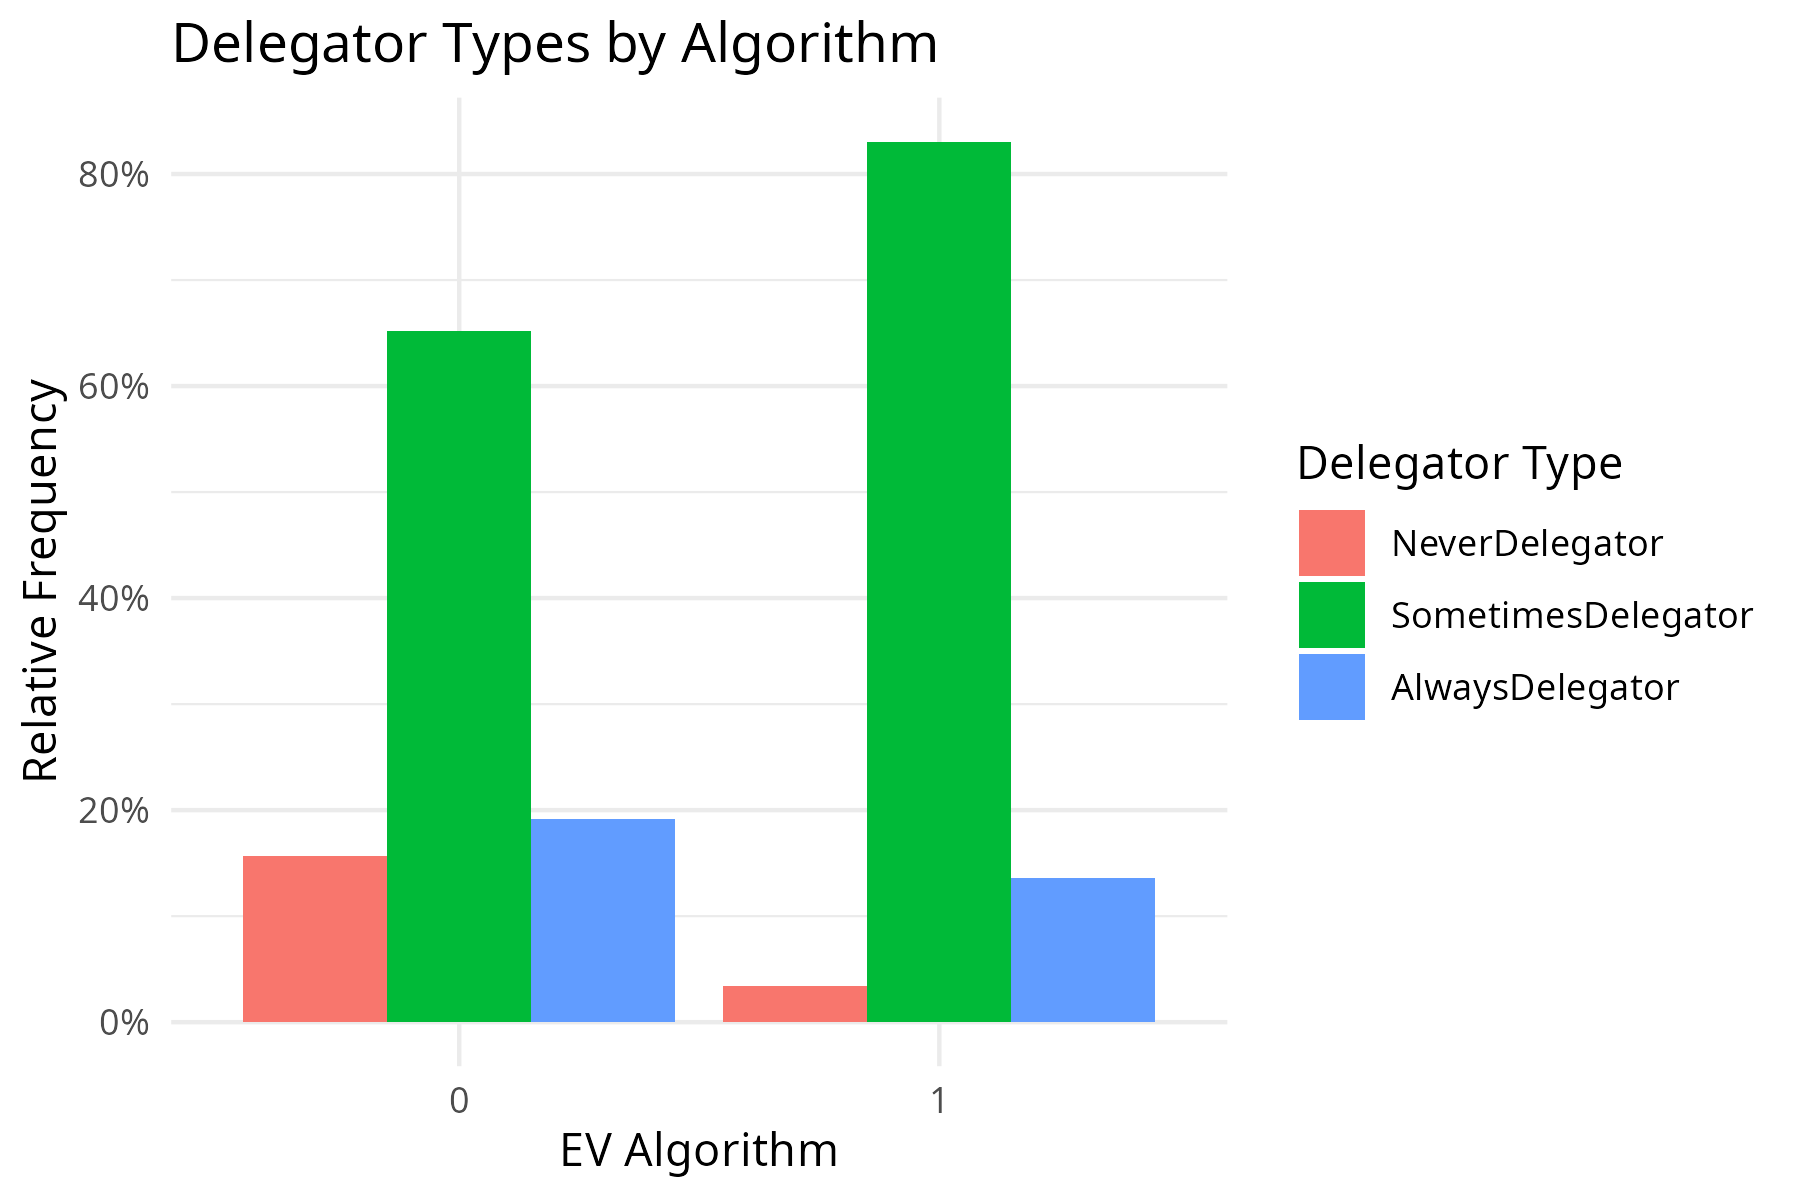
\includegraphics[width=0.78\textwidth]{DelegatorTypesByTrmt.png}
% 	\caption{Distribution of delegator types across treatments (never-delegators vs. sometimes-delegators vs. always-delegators).}
% 	\label{fig:delegation_groups}
% \end{figure}


\subsection{Responses to feedback}
This preregistered secondary analysis characterizes behavioral dynamics rather than serving as an additional primary test of H1.

To characterize feedback dynamics, we estimate a win-stay/lose-shift model on rounds 2--8, regressing an indicator for staying with the same delegation/non-delegation choice on a prior win (a previous-round payoff larger than zero), with task and decision-number fixed effects and participant-clustered standard errors. A prior win is strongly associated with staying ($\beta_{\text{lagWin}}$ = 0.169, SE = 0.035, $p < 0.001$), and this win-stay/lose-shift tendency is statistically indistinguishable across treatments (EVAlgorithm $\times$ lagWin: $\beta$ = 0.009, SE = 0.049, $p = 0.857$). Participants in the EV condition stay somewhat less overall ($\beta_{\text{EVAlgorithm}}$ = $-0.105$, SE = 0.050, $p = 0.036$). In other words, both treatments display the same basic pattern: after a loss, participants are more likely to switch their delegation decision.

A more revealing picture emerges when we distinguish \emph{who} produced the prior outcome---that is, whether the previous round was delegated (so that ``the algorithm lost'') or self-chosen. Estimating the model separately by treatment and interacting a prior loss with prior delegation, the prior-loss\,$\times$\,prior-delegation interaction is negative and significant in both conditions (EV: $\beta$ = $-0.185$, SE = 0.070, $p = 0.009$; preference-based: $\beta$ = $-0.140$, SE = 0.064, $p = 0.030$). That is, a loss prompts more switching in general, but a loss that the algorithm produced prompts substantially more switching than a self-inflicted loss. This is visible in the raw stay rates: after a delegated loss, the stay rate is the lowest in both conditions (54.7\% in the preference-based and 44.4\% in the EV condition), well below the stay rate after a delegated win (78.5\% and 69.7\%) and even below that after a self-chosen loss (67.7\% and 58.3\%). 

This pattern connects to the broader finding that algorithmic mistakes tend to be forgiven less readily than one's own \citep{Dietvorst2018,Renier2021}: participants abandon delegation disproportionately after the algorithm delivers a bad outcome, even though delegated choices were on average substantially more profitable. The dynamics are therefore similar across treatments and reinforce the broader message that the treatment difference is concentrated at first contact, rather than in how participants respond to feedback thereafter.

\subsection{Exploratory mechanisms: post-task reasons and interpretations}
\label{sec:exploratory_mechanisms}
To better understand the behavioral patterns above, we analyze participants' self-reported reasons collected after Part 2. Specifically, after the incentivized rounds, participants indicated whether they would delegate in 10 hypothetical additional tasks and then reported reasons for that hypothetical choice (closed-item checklist plus open text). We treat these responses as exploratory mechanism evidence. Figure \ref{fig:reason_selection} shows reason-selection frequencies by treatment and delegation type.

\begin{figure}[tb]
	\centering
	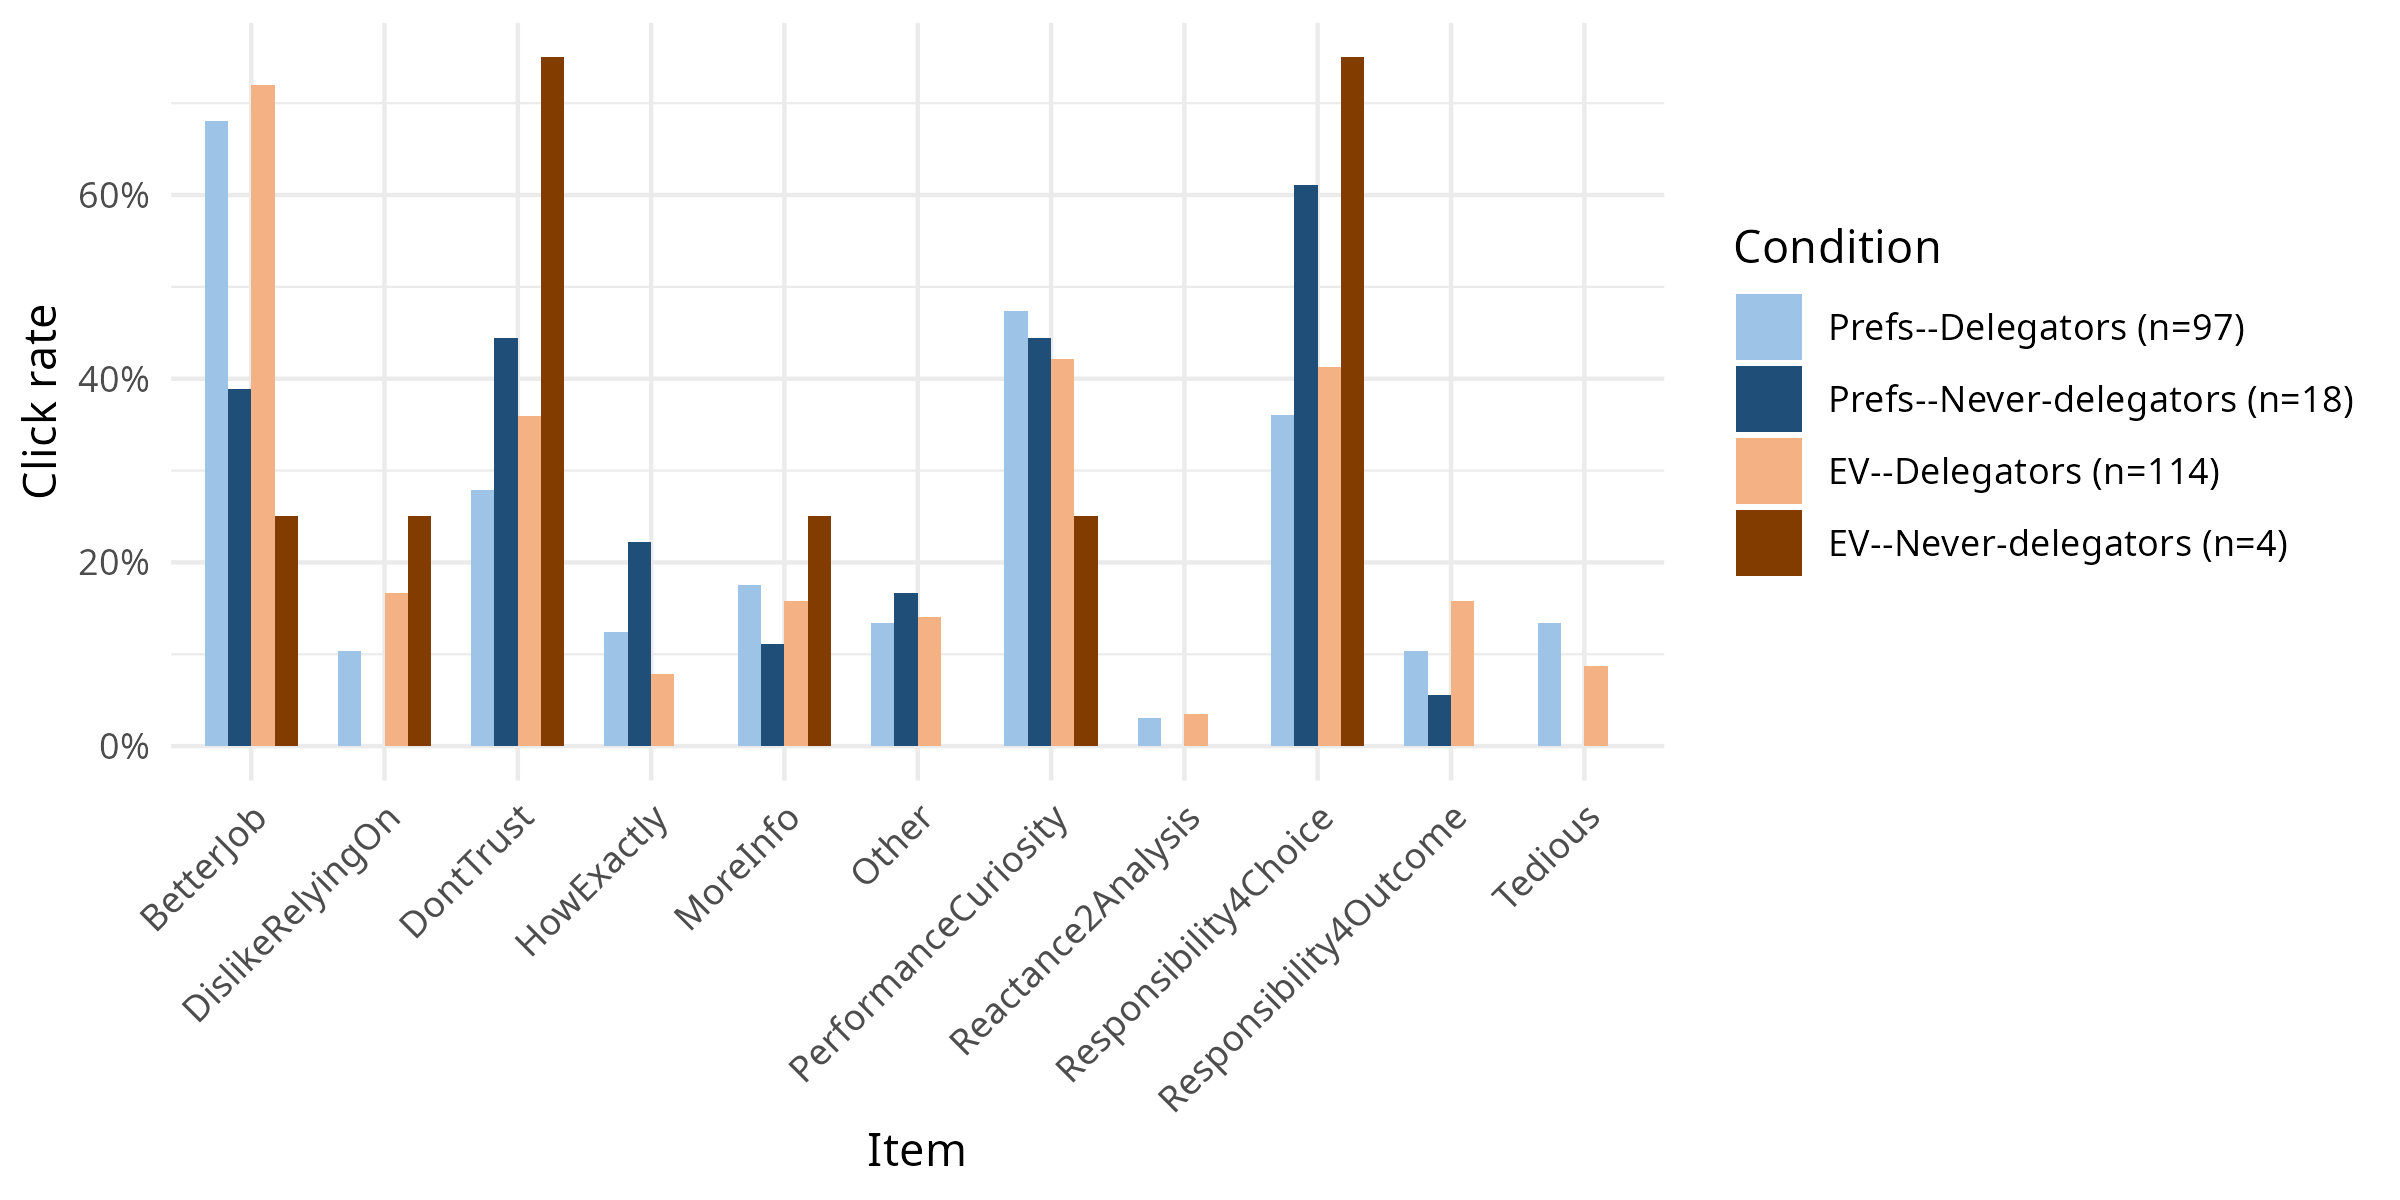
\includegraphics[width=\textwidth]{ReasonsByTrmtAndNeverDelegator2.png}
	\caption{Reasons for hypothetical delegation choices by treatment and delegation type. {\footnotesize Note: After choosing (not) to delegate, participants answered the following items. For paired wordings, the first phrasing corresponds to choosing delegation and the phrasing in parentheses to choosing no delegation: \textit{BetterJob}: I thought the computer could do a better job than me (I could do a better job than the computer); \textit{DislikeRelyingOn}: I don't like relying on myself (computers); \textit{DontTrust}: I don't fully trust myself (the computer); \textit{HowExactly}: I find it unpleasant that I don't know how exactly the computer chooses an option for me; \textit{MoreInfo}: I would have preferred more information about how the computer makes its decisions; \textit{Other}: Other (please specify below); \textit{PerformanceCuriosity}: I wanted to see how well the computer (I) can do; \textit{Reactance2Analysis}: I don't like to be analysed by an algorithm; \textit{Responsibility4Choice}: I didn't want (wanted) to be responsible for choosing an (the) option; \textit{Responsibility4Outcome}: I didn't want to be responsible if a low payment results; \textit{Tedious}: Doing it myself would have been too tedious.}}
	\label{fig:reason_selection}
\end{figure}

The first thing to note is that reason-selection patterns vary more by delegation type than by treatment. The only visible treatment contrast is that differences between never-delegators and delegators appear larger in the EV condition than in the preference-based condition. We do not interpret this contrast because the never-delegator subgroup in the EV condition is very small (4 participants).

Two descriptive patterns are consistent with the behavioral results. First, participants who delegated (at least once) were more likely to indicate performance-based motives (on average, 70.1\% indicated that the computer would choose better, while only 36.4\% of the never-delegators indicated this). Second, participants who never delegated were more likely to select reasons centered on distrust of the algorithm (32.2\% vs. 50\%) and retaining personal responsibility for the choice (38.9\% vs. 63.6\%). This mirrors the treatment-level non-delegator pattern and is consistent with the idea that a subgroup places relatively more weight on agency and responsibility concerns than on expected performance.

Exploratory interaction models lend quantitative support to treatment-specific deterrence channels (Figure~\ref{fig:coef_bad_absurd} in the appendix). In a linear probability model of individual delegation decisions interacting treatment with participants' algorithmic performance expectations (controlling for decision round, per-choice Part-1 confidence, revealed Part-1 risk preferences, and task fixed effects), the non-preferred-choices estimate is strongly negatively associated with delegation in the preference-based condition ($\beta = -0.058$, SE = 0.016, $p < 0.001$) and substantially attenuated in the EV condition (EVAlgorithm $\times$ non-preferred: $\beta = +0.035$, SE = 0.020, $p = 0.090$). Conversely, the completely-weird-choices estimate shows near-zero association with delegation in the preference-based condition ($\beta = +0.007$, SE = 0.018, $p = 0.709$) but is strongly and negatively associated with delegation in the EV condition (EVAlgorithm $\times$ completely weird: $\beta = -0.070$, SE = 0.023, $p = 0.003$). This pattern suggests that what deters delegation differs by algorithm type: perceived non-preferred choices are a deterrent specifically under personalization, while perceived extreme errors (completely weird choices) are a deterrent under objective optimization.

Importantly, the expectation data also speak directly to a natural concern about our manipulation---namely, whether participants believed that the preference-based algorithm actually captured their preferences. They did: participants in the preference-based condition expected the algorithm to make significantly \emph{fewer} non-preferred choices than participants in the EV condition (on average 3.78 out of 10 vs. 5.00 out of 10; $t = -4.15$, $p < 0.001$; Wilcoxon rank-sum $p < 0.001$; Figure~\ref{fig:expected_bad_absurd}). In other words, the personalized algorithm was credited with doing its job of matching participants' preferences. By contrast, expectations about ``completely weird'' choices did not differ meaningfully across conditions (1.57 vs. 1.78; $t = -0.94$, $p = 0.351$). This makes the reduced delegation under personalization all the more striking: even though participants believed the preference-based algorithm would more often pick options in line with their preferences, they were not more---and at first contact were less---willing to delegate to it. This is consistent with the interpretation that the barrier to delegating to the personalized algorithm lies not in doubts about its accuracy but in concerns about ceding choice authority. It also fits the observation that the two explanation-demand items (wanting to know how exactly the computer chooses, and wanting more information about how it decides) were selected only infrequently: participants' reservations were not primarily about understanding or trusting the algorithm's competence at preference-matching.

Additional reason items are informative by contrast. Items such as not wanting to be analyzed by an algorithm were rarely selected overall, reinforcing that opacity- and profiling-related concerns were unlikely to be primary drivers of treatment differences in this setting. By comparison, selecting the task being tedious appears more among delegators (though still at a low level, 10.9\% vs. 0\%), consistent with an effort-saving channel among participants who are willing to hand over control. Open-text responses also repeatedly mention time press

These mechanism patterns have to be interpreted cautiously. The reason measures are ex-post and refer to the hypothetical additional choice rather than the incentivized rounds themselves. They therefore function as suggestive proxies for motives, not as causal identification of psychological channels or as decisive evidence for one mechanism over another.

%Given multiple supplementary contrasts, these exploratory estimates should be interpreted cautiously and with emphasis on effect magnitude and directional consistency rather than on single p-values.




%\begin{figure}[htbp]
%\centering
%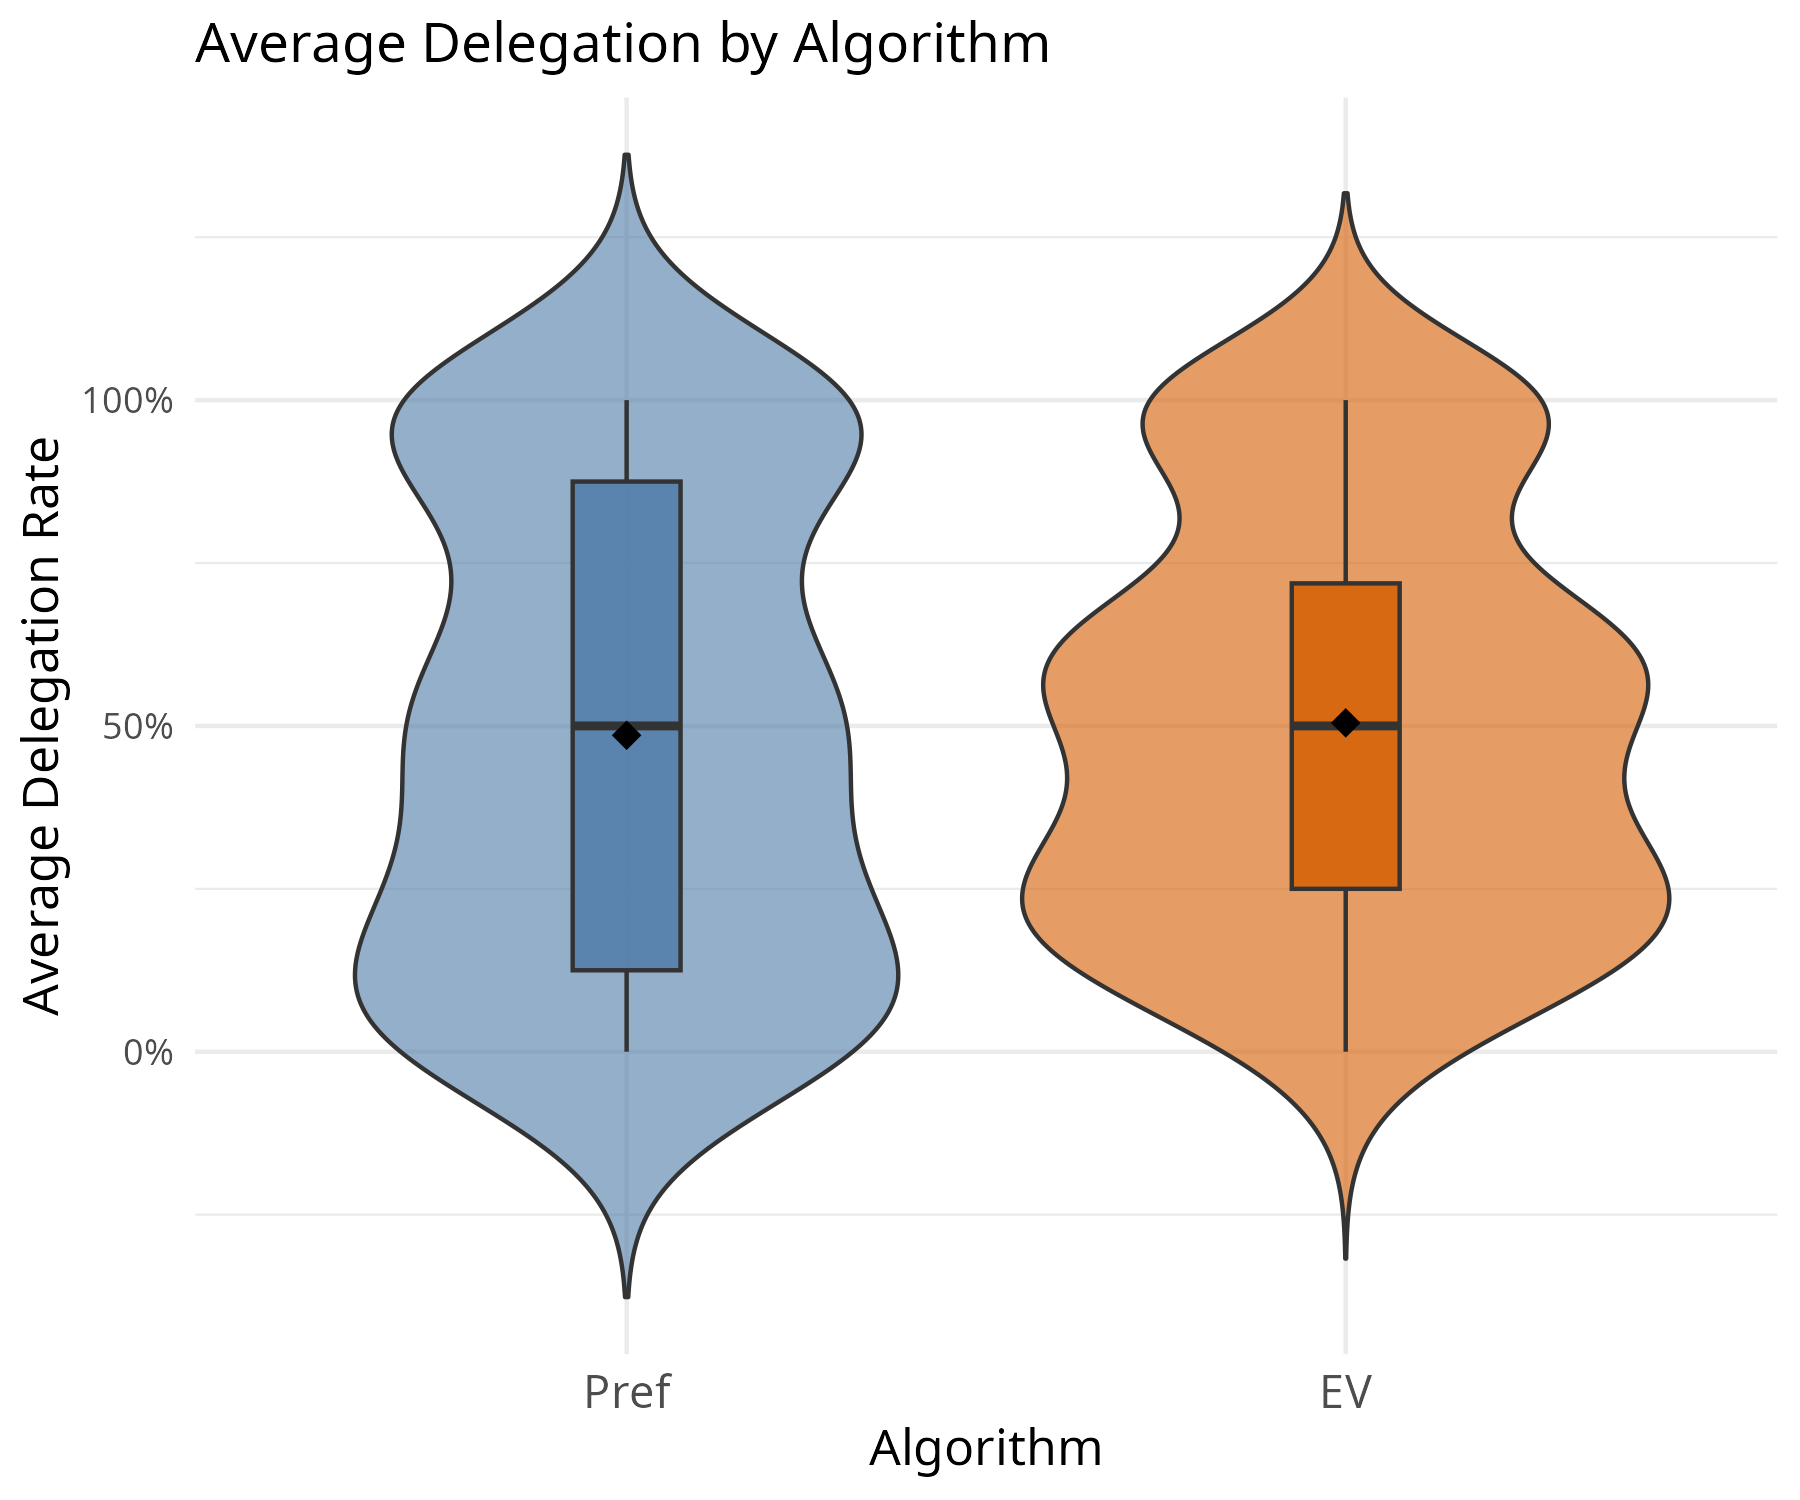
\includegraphics[width=0.78\textwidth]{Figure2_DistributionDelegation.png}
%\caption{Distribution of delegation propensities across participants.}
%\label{fig:delegation_distribution}
%\end{figure}


\section{Discussion}
\label{sec:discussion}

\subsection{Core finding}
This preregistered study shows that preference-based personalization can deter delegation rather than increase it. We observe this deterrence in two forms: lower delegation at first contact and a larger subgroup of participants who never delegate under personalization.

The first-contact finding is important because it captures behavior before participants can learn from outcome feedback. At that stage, delegation is driven primarily by how participants interpret the algorithmic rule itself. Our evidence is consistent with the interpretation that an impersonal EV rule is initially easier to accept as a legitimate external computation than a profile-based personalized rule based on the user's own revealed preferences. Even though subsequent rounds show convergence in average delegation, first-contact differences remain practically important because initial adoption decisions can have path-dependent downstream effects in real-world deployment (e.g., immediate opt-out, lower willingness to return, and weaker opportunity for learning-by-use).

\subsection{Interpretation and relation to prior work}
Our main contribution is to show that algorithm uptake depends on the decision rule, not just on whether a system is algorithmic. The contrast between expected-value maximization and preference-based personalization indicates that users may resist personalization despite its normative appeal.

The categorical non-delegation pattern is particularly informative: many participants entirely avoid delegation under personalization, consistent with work on autonomy, responsibility, and control as drivers of acceptance. Exploratory post-task reasons (Section~\ref{sec:exploratory_mechanisms}) align with this interpretation, especially the stronger emphasis among never-delegators on responsibility and distrust, while concerns about being algorithmically analyzed appear comparatively rare. Because these reason measures are ex-post and hypothetical, this evidence remains suggestive rather than causal. The exploratory expectation data also indicate that treatment differences in anticipated non-preferred and completely weird choices are modest, so mechanism differences are better interpreted as differences in how these expectations map into delegation than as large between-treatment expectation gaps.

These findings are consistent with an earlier study on the same question (reported as a chapter in Suraci's PhD thesis), which motivated and informed the design of the present preregistered experiment. In that study, the delegation gap between EV and preference-based treatments was larger (about 20 percentage points) and persisted over decisions. Recomputing the categorical non-delegation contrast for that earlier sample also yields a significant difference (32/189 in preference-based treatments vs. 17/187 in EV treatments; one-sided Boschloo exact test, $p = 0.0135$).\footnote{Note that categorical non-delegation was not analyzed or reported in the earlier study, which is the reason for why we did not pre-register its analysis for the present study.}

\subsection{Limitations}
The findings should be interpreted in light of several limitations. First, the study is an online experiment with stylized financial lotteries, so external validity to field settings should be interpreted cautiously. Second, although behavioral outcomes are well suited for studying reliance, the design does not causally identify the psychological mechanism behind first-contact hesitation or categorical non-delegation (e.g., perceived objectivity, profiling concerns, or accountability salience). Third, the present analyses focus on short-run repeated interaction; longer-run adaptation to personalized systems remains an open question.

\subsection{Implications and future research}
For design, the results imply that personalization should not be treated as a uniformly beneficial acceptance lever. In settings where objective criteria are salient and normatively legitimate, objective optimization may face lower initial resistance than preference-based personalization. This has direct implications for the design and communication of decision aids in finance and other high-stakes domains.

These implications extend beyond our experimental setting. Financial robo-advisors routinely face the choice between objective portfolio rules (e.g., mean-variance optimization) and preference-based personalization derived from risk profiling questionnaires \citep{Capponi2022,Ruehr2020}. Our findings suggest that the very feature intended to increase subjective fit---tailoring the algorithm to the user's profile---may inadvertently encroach on users' sense of choice authority, deterring precisely those users who value exercising active control over their decisions. The same tension arises whenever algorithmic decision aids must be voluntarily adopted: in healthcare, treatment recommender systems can follow clinical-evidence guidelines or patient-preference protocols; in hiring, screening tools can apply standardized criteria or adaptively weight candidate profiles. In each case, the assumption that preference alignment promotes adoption deserves empirical scrutiny rather than being taken as a design axiom.

Future research should test mechanism-targeted interventions at first contact, including reframing of personalization logic, responsibility framing, and alternative explanation formats. It should also examine whether the non-delegator subgroup is stable across domains, stakes, and cultural contexts.

\subsection{Contributions}
This paper makes three contributions. First, it provides preregistered evidence that personalization can reduce, rather than increase, delegation at first contact. Second, it shows that resistance is not only transient: personalization is associated with substantially more categorical non-delegation. Third, by comparing two algorithmic decision rules within the same task, it clarifies that behavioral uptake depends on perceived rule characteristics, not only on whether advice is algorithmic or human.

\subsection{Data and code availability}
Data, analysis code, and study materials will be deposited in a public repository upon acceptance/publication of this manuscript. %During peer review, the replication package is maintained in a private repository and will be unblinded and made publicly accessible after acceptance.

%Declaration of generative AI use
%Authors must declare the use of generative AI in the manuscript preparation process upon submission of the paper.
%
%Elsevier recognizes the potential of generative AI and AI-assisted technologies (“AI Tools”), when used responsibly, to help researchers work efficiently, gain critical insights fast and achieve better outcomes. Increasingly, these tools, including AI agents and deep research tools, are helping researchers to synthesize complex literature, provide an overview of a field or research question, identify research gaps, generate ideas, and provide tailored support for tasks such as content organization and improving language and readability.
%
%Authors preparing a manuscript for this journal can use AI Tools to support them. However, these tools must never be used as a substitute for human critical thinking, expertise and evaluation. AI technology should always be applied with human oversight and control.
%
%Ultimately, authors are responsible and accountable for the contents of their work. This includes accountability for:
%
%Carefully reviewing and verifying the accuracy, comprehensiveness, and impartiality of all AI-generated output (including checking the sources, as AI-generated references can be incorrect or fabricated).
%
%Editing and adapting all material thoroughly to ensure the manuscript represents the author’s authentic and original contribution and reflects their own analysis, interpretation, insights and ideas.
%
%Ensuring the use of any tools or sources, AI-based or otherwise, is made clear and transparent to readers. If AI Tools have been used, we require a disclosure statement upon submission; please see example below.
%
%Ensuring the manuscript is developed in a way that safeguards data privacy, intellectual property and other rights, by checking the terms and conditions of any AI tool that is used.
%
%Finally, authors must not list or cite AI Tools as an author or co-author on the manuscript since authorship implies responsibilities and tasks that can only be attributed to, and performed by, humans.
%
%The use of AI Tools in the manuscript preparation process must be declared by adding a statement at the end of the manuscript when the paper is first submitted. The statement will appear in the published work and should be placed in a new section before the references list.
%
%An example:
%
%Title of new section: 
\subsection{Declaration of generative AI and AI-assisted technologies in the manuscript preparation process}

During the preparation of this work the authors used [NAME OF TOOL / SERVICE] in order to [REASON]. After using this tool/service, the authors reviewed and edited the content as needed and take full responsibility for the content of the published article.

%The declaration does not apply to the use of basic tools, such as tools used to check grammar, spelling and references. If you have nothing to disclose, you do not need to add a statement.
%
%Please read Elsevier’s author policy on the use of generative AI and AI-assisted technologies, which can be found in the generative AI policies for journals.
%
%Please note: to protect authors’ rights and the confidentiality of their research, this journal does not currently allow the use of generative AI or AI-assisted technologies such as ChatGPT or similar services by reviewers or editors in the peer review and manuscript evaluation process, as is stated in Elsevier's generative AI policies for journals. Elsevier is actively evaluating compliant AI Tools and may revise this policy in the future.


\newpage
\thispagestyle{plain}
\addtolength{\topmargin}{-.5cm}
\addtolength{\textheight}{.8cm}

%% \begin{appendices}
% % {\startsupplement
% \renewcommand{\thesection}{Appendix \Alph{section}}
%\renewcommand{\thesubsection}{%\Alph{section}.
%\Roman{subsection}}
\renewcommand{\thefigure}{\Alph{section}.\arabic{figure}}% \Alph{section}}
%\renewcommand{\thetable}{\Alph{section}.\arabic{table}}
\setcounter{section}{1}
\setcounter{figure}{0}
%\thispagestyle{plain}

\section*{Appendix}

\begin{figure}[htbp]
\centering
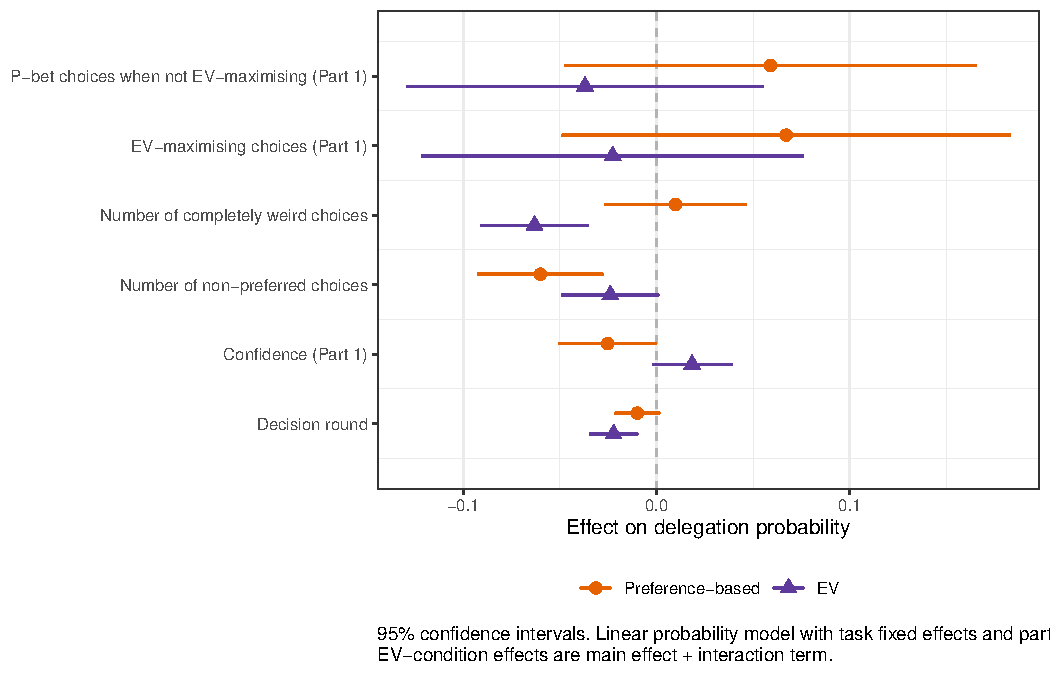
\includegraphics[width=0.75\textwidth]{CoefPlotBadAbsurd.pdf}
\caption{Condition-specific marginal effects on delegation probability. The plot shows all regression coefficients from the linear probability model (main effects and treatment interactions). Key expectation variables include the participant's expectation about the number of non-preferred choices (out of 10) and about the number of ``completely weird'' choices (out of 10). The preference-based-condition estimate is the main-effect coefficient; the EV-condition estimate is the sum of the main effect and the treatment interaction term. Error bars are 95\% confidence intervals based on participant-clustered standard errors. The model controls for decision round, per-choice Part-1 confidence, revealed Part-1 risk preferences (a combination of the number of EV-maximising choices in Part 1 and the number of choices that were less risky in the sense of having fewer states with a payoff of 0 amongst those choices in which this less risky choice was not simultaneously the EV-maximising choice), and task fixed effects.}
\label{fig:coef_bad_absurd}
\end{figure}
\clearpage
\begin{figure}[tb]
\centering
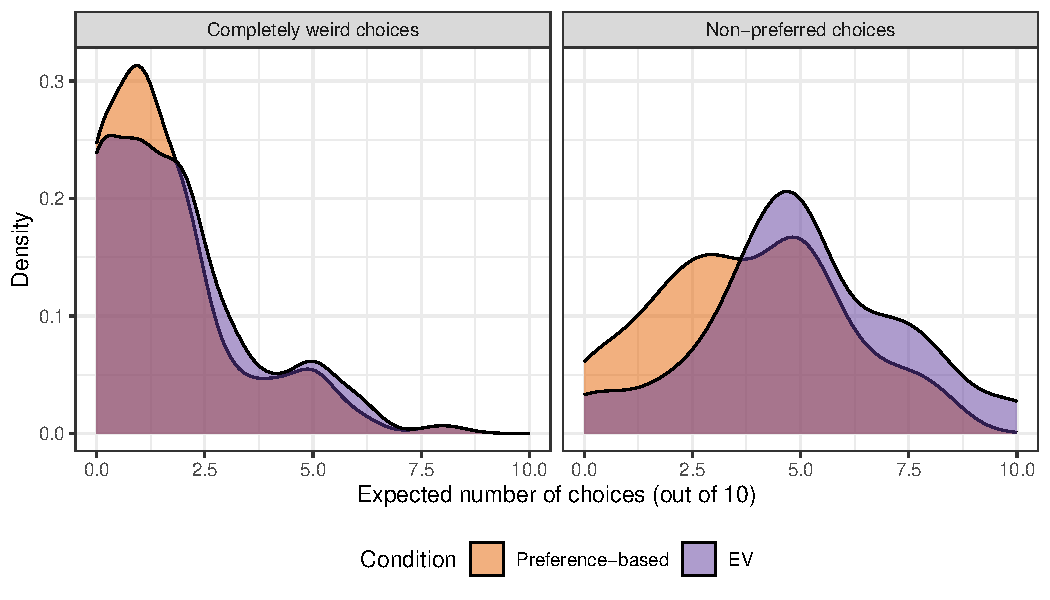
\includegraphics[width=0.75\textwidth]{ExpectedBadAndAbsurdChoicesByTrmt.pdf}
\caption{Distribution of expected algorithmic non-preferred and completely weird choices by treatment. The figure shows descriptive densities of participants' post-task expectations for both variables, separately for the preference-based and EV conditions.\vspace{.5cm}}
\label{fig:expected_bad_absurd}
\end{figure}

\bibliographystyle{apalike}
\bibliography{library}

\end{document}
